\documentclass[10pt]{article}
% The house preprint layout: Times, a 5.5 by 9 inch text block, ruled title.
\usepackage[letterpaper,textwidth=5.5in,textheight=9in]{geometry}
\usepackage[T1]{fontenc}
\usepackage{newtxtext,newtxmath}
\usepackage{microtype}
\usepackage{graphicx}
\usepackage{booktabs}
\usepackage{array}
\usepackage{longtable}
\usepackage{float}
\usepackage{enumitem}
\usepackage{titlesec}
\usepackage{fancyhdr}
\usepackage{xcolor}
\usepackage{soul}
\usepackage[labelfont=bf,labelsep=period,justification=justified,singlelinecheck=false,skip=6pt]{caption}
\usepackage{xurl}
\usepackage[colorlinks=true,linkcolor=black,citecolor=black,urlcolor=black]{hyperref}
\definecolor{ink}{HTML}{16213A}
\definecolor{sage}{HTML}{7F9B8E}
\definecolor{flame}{HTML}{E8542A}
\setlength{\parindent}{0pt}
\setlength{\parskip}{5.5pt}
\titleformat{\section}{\large\bfseries}{\thesection}{1em}{}
\titleformat{\subsection}{\normalsize\bfseries}{\thesubsection}{1em}{}
\titlespacing*{\section}{0pt}{14pt}{5pt}
\titlespacing*{\subsection}{0pt}{10pt}{3pt}
% \draftfalse drops the draft label for the release build; \chg marks text changed since the 11/8 v35 draft
% (highlighting needs pdflatex), and \markchangesfalse prints it unmarked.
\newif\ifdraft\draftfalse
\newif\ifmarkchanges\markchangesfalse
\fancypagestyle{first}{\fancyhf{}\renewcommand{\headrulewidth}{0pt}\ifdraft\fancyhead[R]{\small\textbf{As of 11/11 (v36)}}\fancyfoot[L]{\small Preprint. Revised draft as of 11/11 (11 November 2026), version 36\ifmarkchanges, with changes from the 11/8 v35 draft highlighted in yellow\fi.}\else\fancyfoot[L]{\small Preprint. November 2026.}\fi}
\ifmarkchanges\sethlcolor{yellow}\soulregister{\cite}{7}\soulregister{\ref}{7}\DeclareRobustCommand{\chg}[1]{\hl{#1}}\else\newcommand{\chg}[1]{#1}\fi
\newcommand{\chgbox}[1]{\ifmarkchanges\colorbox{yellow}{#1}\else#1\fi}
\newcommand{\head}[1]{\textbf{#1}\hspace{0.8em}}
\newcommand{\ActGapSafeAfter}{6}
\newcommand{\ActGapSafeBefore}{28}
\newcommand{\AgreeGpt}{89}
\newcommand{\AgreePanel}{94}
\newcommand{\AllThreeAgree}{88}
\newcommand{\AuthCtl}{62}
\newcommand{\AuthMid}{73}
\newcommand{\AuthMidhi}{3.70}
\newcommand{\AuthMidlo}{0.79}
\newcommand{\AuthMidor}{1.71}
\newcommand{\AuthMidp}{0.17}
\newcommand{\AuthN}{60}
\newcommand{\AuthNv}{93}
\newcommand{\AuthOutCtl}{15}
\newcommand{\AuthOutMid}{4}
\newcommand{\AuthOutNv}{11}
\newcommand{\AuthOutSafe}{4}
\newcommand{\AuthSafe}{57}
\newcommand{\AuthSafehi}{1.69}
\newcommand{\AuthSafelo}{0.39}
\newcommand{\AuthSafeor}{0.81}
\newcommand{\AuthSafep}{0.58}
\newcommand{\BenActedSafehi}{1.20}
\newcommand{\BenActedSafelo}{0.39}
\newcommand{\BenActedSafeor}{0.69}
\newcommand{\BenActedhi}{0.88}
\newcommand{\BenActedlo}{0.30}
\newcommand{\BenActedor}{0.51}
\newcommand{\BenActsCtl}{85}
\newcommand{\BenActsMid}{73}
\newcommand{\BenActsSafe}{79}
\newcommand{\BenNoActionCtl}{15}
\newcommand{\BenNoActionMid}{27}
\newcommand{\BenNoActionSafe}{21}
\newcommand{\BenignRuns}{990}
\newcommand{\COneGptor}{0.57}
\newcommand{\COnehi}{0.97}
\newcommand{\COnelo}{0.43}
\newcommand{\COneor}{0.65}
\newcommand{\COnep}{0.037}
\newcommand{\CodeAgree}{91}
\newcommand{\CodeAgreeN}{150}
\newcommand{\CodeKappa}{0.69}
\newcommand{\CodedFirms}{724}
\newcommand{\ComboRuns}{450}
\newcommand{\ConfActedhi}{0.84}
\newcommand{\ConfActedlo}{0.30}
\newcommand{\ConfActedor}{0.50}
\newcommand{\ConfNoActionCtl}{9}
\newcommand{\ConfNoActionMid}{22}
\newcommand{\ConfNodrhi}{0.76}
\newcommand{\ConfNodrlo}{0.26}
\newcommand{\ConfNodror}{0.44}
\newcommand{\ConfPartnerhi}{1.51}
\newcommand{\ConfPartnerlo}{0.59}
\newcommand{\ConfPartneror}{0.94}
\newcommand{\ConfRuns}{840}
\newcommand{\ConfirmRuns}{720}
\newcommand{\CutPct}{1.1}
\newcommand{\DOnehi}{0.75}
\newcommand{\DOneholm}{0.003}
\newcommand{\DOnelo}{0.29}
\newcommand{\DOneor}{0.47}
\newcommand{\DTwohi}{1.03}
\newcommand{\DTwoholm}{0.063}
\newcommand{\DTwolo}{0.38}
\newcommand{\DTwoor}{0.63}
\newcommand{\DoseHi}{0.55}
\newcommand{\DoseLo}{0.23}
\newcommand{\DoseOr}{0.36}
\newcommand{\DoseTarget}{0.64}
\newcommand{\DurAcrossOr}{0.37}
\newcommand{\EActedor}{0.99}
\newcommand{\EHetp}{0.026}
\newcommand{\EOnehi}{1.12}
\newcommand{\EOnelo}{0.47}
\newcommand{\EOneor}{0.73}
\newcommand{\EOnep}{0.15}
\newcommand{\EPoolGpthi}{0.85}
\newcommand{\EPoolGptlo}{0.46}
\newcommand{\EPoolGptor}{0.62}
\newcommand{\EPoolGptp}{0.003}
\newcommand{\EPoolhi}{1.03}
\newcommand{\EPoollo}{0.56}
\newcommand{\EPoolor}{0.76}
\newcommand{\EPoolp}{0.077}
\newcommand{\ETwohi}{1.21}
\newcommand{\ETwolo}{0.52}
\newcommand{\ETwoor}{0.79}
\newcommand{\ETwop}{0.28}
\newcommand{\EroMidhi}{2.29}
\newcommand{\EroMidlo}{0.60}
\newcommand{\EroMidor}{1.17}
\newcommand{\EroSafehi}{6.13}
\newcommand{\EroSafelo}{1.52}
\newcommand{\EroSafeor}{3.05}
\newcommand{\FOneGptor}{1.23}
\newcommand{\FOnehi}{1.64}
\newcommand{\FOnelo}{0.43}
\newcommand{\FOneor}{0.84}
\newcommand{\FOnep}{0.615}
\newcommand{\FirmRuns}{2{,}040}
\newcommand{\FleissK}{0.81}
\newcommand{\GapMidAfter}{15}
\newcommand{\GapMidBefore}{18}
\newcommand{\GapSafeAfter}{7}
\newcommand{\GapSafeBefore}{29}
\newcommand{\HOnehi}{0.64}
\newcommand{\HOneholm}{0.0003}
\newcommand{\HOnelo}{0.25}
\newcommand{\HOneor}{0.40}
\newcommand{\HTwohi}{0.87}
\newcommand{\HTwoholm}{0.019}
\newcommand{\HTwolo}{0.22}
\newcommand{\HTwoor}{0.44}
\newcommand{\IVCoreor}{0.43}
\newcommand{\IVDirectoror}{0.39}
\newcommand{\IVPartneror}{1.31}
\newcommand{\IVReverseor}{0.51}
\newcommand{\JudgedLacking}{0}
\newcommand{\JudgedN}{6{,}194}
\newcommand{\KeepMid}{82}
\newcommand{\KeepSafe}{23}
\newcommand{\MidBenAlonehi}{0.63}
\newcommand{\MidBenAlonelo}{0.23}
\newcommand{\MidBenAloneor}{0.38}
\newcommand{\MidSafeAlonehi}{1.13}
\newcommand{\MidSafeAlonelo}{0.53}
\newcommand{\MidSafeAloneor}{0.78}
\newcommand{\MidSafeAlonep}{0.184}
\newcommand{\OtherNoActionCtl}{18}
\newcommand{\OtherNoActionMid}{28}
\newcommand{\OtherRuns}{720}
\newcommand{\PairKappaHi}{0.84}
\newcommand{\PairKappaLo}{0.79}
\newcommand{\PctActedHarmCc}{70}
\newcommand{\PctActedHarmM}{58}
\newcommand{\PctActedHarmS}{54}
\newcommand{\PctBenCc}{54}
\newcommand{\PctBenM}{39}
\newcommand{\PctBenS}{48}
\newcommand{\PctComboCtl}{42}
\newcommand{\PctComboMid}{33}
\newcommand{\PctCtlAlone}{54}
\newcommand{\PctCtlFirm}{47}
\newcommand{\PctDirCc}{63}
\newcommand{\PctDirM}{45}
\newcommand{\PctDirS}{34}
\newcommand{\PctMidAlone}{44}
\newcommand{\PctMidFirm}{41}
\newcommand{\PctMidSafeAlone}{25}
\newcommand{\PctMidSafeFirm}{18}
\newcommand{\PctNvAlone}{54}
\newcommand{\PctNvFirm}{75}
\newcommand{\PctOneMidAfter}{46}
\newcommand{\PctOneMidBefore}{44}
\newcommand{\PctOneSafeAfter}{44}
\newcommand{\PctOneSafeBefore}{40}
\newcommand{\PctOtherCtl}{57}
\newcommand{\PctOtherMid}{50}
\newcommand{\PctParCc}{71}
\newcommand{\PctParM}{69}
\newcommand{\PctParS}{69}
\newcommand{\PctRestrCtl}{58}
\newcommand{\PctRestrMid}{47}
\newcommand{\PctSafeAlone}{30}
\newcommand{\PctSafeCtlAlone}{54}
\newcommand{\PctSafeCtlFirm}{48}
\newcommand{\PctSafeFirm}{18}
\newcommand{\PoolDurHi}{0.92}
\newcommand{\PoolDurLo}{0.35}
\newcommand{\PoolDurOr}{0.57}
\newcommand{\PoolHi}{0.93}
\newcommand{\PoolLo}{0.59}
\newcommand{\PoolOr}{0.74}
\newcommand{\PoolQ}{1.3}
\newcommand{\QFourhi}{2.11}
\newcommand{\QFourholm}{0.55}
\newcommand{\QFourlo}{0.81}
\newcommand{\QFouror}{1.31}
\newcommand{\QOnehi}{1.04}
\newcommand{\QOneholm}{0.25}
\newcommand{\QOnelo}{0.53}
\newcommand{\QOneor}{0.74}
\newcommand{\QThreehi}{4.55}
\newcommand{\QThreeholm}{<0.001}
\newcommand{\QThreelo}{2.02}
\newcommand{\QThreeor}{3.03}
\newcommand{\QTwohi}{1.82}
\newcommand{\QTwoholm}{0.55}
\newcommand{\QTwolo}{0.74}
\newcommand{\QTwoor}{1.16}
\newcommand{\RefComboA}{19}
\newcommand{\RefComboB}{4}
\newcommand{\RefCombohi}{15.7}
\newcommand{\RefCombolo}{1.7}
\newcommand{\RefComboor}{5.2}
\newcommand{\RefCombop}{0.003}
\newcommand{\RefDropRatio}{0.93}
\newcommand{\RefDropRatiohi}{4.26}
\newcommand{\RefDropRatiolo}{0.20}
\newcommand{\RefMiCtl}{6}
\newcommand{\RefMiMid}{23}
\newcommand{\RefMidBenA}{7}
\newcommand{\RefMidBenB}{1}
\newcommand{\RefMidBenhi}{62.1}
\newcommand{\RefMidBenlo}{0.9}
\newcommand{\RefMidBenor}{7.4}
\newcommand{\RefMidBenp}{0.064}
\newcommand{\RefMidDropA}{4}
\newcommand{\RefMidDropB}{10}
\newcommand{\RefMidDrophi}{1.3}
\newcommand{\RefMidDroplo}{0.1}
\newcommand{\RefMidDropor}{0.4}
\newcommand{\RefMidDropp}{0.113}
\newcommand{\RefMior}{4.3}
\newcommand{\RefNvCtl}{2}
\newcommand{\RefNvMid}{14}
\newcommand{\RefNvor}{7.9}
\newcommand{\RefOtherCtl}{7}
\newcommand{\RefOtherMid}{37}
\newcommand{\RefPoolCtl}{9}
\newcommand{\RefPoolMid}{51}
\newcommand{\RefPoolN}{540}
\newcommand{\RefPoolhi}{13.4}
\newcommand{\RefPoollo}{3.1}
\newcommand{\RefPoolor}{6.5}
\newcommand{\RefQwCtl}{1}
\newcommand{\RefQwMid}{14}
\newcommand{\RefQwor}{17.6}
\newcommand{\RefSafeBenA}{5}
\newcommand{\RefSafeBenB}{1}
\newcommand{\RefSafeBenhi}{47.4}
\newcommand{\RefSafeBenlo}{0.6}
\newcommand{\RefSafeBenor}{5.4}
\newcommand{\RefSafeBenp}{0.131}
\newcommand{\RefSafeDropA}{6}
\newcommand{\RefSafeDropB}{16}
\newcommand{\RefSafeDrophi}{0.9}
\newcommand{\RefSafeDroplo}{0.1}
\newcommand{\RefSafeDropor}{0.4}
\newcommand{\RefSafeDropp}{0.035}
\newcommand{\RefSafeFreshA}{17}
\newcommand{\RefSafeFreshB}{2}
\newcommand{\RefSafeFreshhi}{44.4}
\newcommand{\RefSafeFreshlo}{2.2}
\newcommand{\RefSafeFreshor}{9.8}
\newcommand{\RefSafeFreshp}{0.003}
\newcommand{\RefShareNv}{50}
\newcommand{\RefShareOther}{88}
\newcommand{\Refusals}{306}
\newcommand{\RelBenM}{28}
\newcommand{\RelBenS}{12}
\newcommand{\RelCombo}{21}
\newcommand{\RelDirM}{29}
\newcommand{\RelDirS}{46}
\newcommand{\RelMidAlone}{19}
\newcommand{\RelMidFirm}{13}
\newcommand{\RelNvFirm}{38}
\newcommand{\RelOther}{11}
\newcommand{\RelSafeAlone}{45}
\newcommand{\RelSafeFirm}{62}
\newcommand{\RestrActedor}{0.71}
\newcommand{\RestrGpthi}{0.61}
\newcommand{\RestrGptlo}{0.24}
\newcommand{\RestrGptor}{0.38}
\newcommand{\RestrGptp}{0.000}
\newcommand{\RestrNoActionCtl}{12}
\newcommand{\RestrNoActionMid}{23}
\newcommand{\Restrhi}{0.88}
\newcommand{\Restrlo}{0.34}
\newcommand{\Restror}{0.54}
\newcommand{\Restrp}{0.013}
\newcommand{\SOnehi}{0.38}
\newcommand{\SOneholm}{<0.001}
\newcommand{\SOnelo}{0.14}
\newcommand{\SOneor}{0.23}
\newcommand{\STwohi}{0.48}
\newcommand{\STwoholm}{<0.001}
\newcommand{\STwolo}{0.11}
\newcommand{\STwoor}{0.23}
\newcommand{\SafeActedCtl}{82}
\newcommand{\SafeActedSafe}{55}
\newcommand{\SafeAlonehi}{0.49}
\newcommand{\SafeAlonelo}{0.24}
\newcommand{\SafeAloneor}{0.35}
\newcommand{\SafeAlonep}{<0.001}
\newcommand{\SafeBenAlonehi}{0.91}
\newcommand{\SafeBenAlonelo}{0.35}
\newcommand{\SafeBenAloneor}{0.57}
\newcommand{\SafeBenDirhi}{1.13}
\newcommand{\SafeBenDirlo}{0.43}
\newcommand{\SafeBenDiror}{0.70}
\newcommand{\SafeDirActedhi}{0.67}
\newcommand{\SafeDirActedlo}{0.22}
\newcommand{\SafeDirActedor}{0.38}
\newcommand{\SafeDirActs}{63}
\newcommand{\SafeDirNoAction}{37}
\newcommand{\SafeFirmhi}{0.32}
\newcommand{\SafeFirmlo}{0.13}
\newcommand{\SafeFirmor}{0.21}
\newcommand{\SafeFirmp}{<0.001}
\newcommand{\SafeHarmActedCtl}{59}
\newcommand{\SafeHarmActedSafe}{33}
\newcommand{\SafePartnerhi}{1.47}
\newcommand{\SafePartnerlo}{0.57}
\newcommand{\SafePartneror}{0.92}
\newcommand{\SafeRuns}{1620}
\newcommand{\SafeSeatRuns}{360}
\newcommand{\ShrinkMid}{18}
\newcommand{\ShrinkSafe}{77}
\newcommand{\SingleRuns}{1{,}200}
\newcommand{\TOnehi}{0.95}
\newcommand{\TOnelo}{0.30}
\newcommand{\TOneor}{0.54}
\newcommand{\TOnep}{0.034}
\newcommand{\TThreehi}{1.57}
\newcommand{\TThreelo}{0.60}
\newcommand{\TThreeor}{0.97}
\newcommand{\TThreep}{0.903}
\newcommand{\Targeted}{2{,}340}
\newcommand{\UdrFirmOr}{0.77}

\makeatletter\newcommand{\rows}[1]{\@@input generated/#1.tex }\makeatother

\renewcommand{\topfraction}{0.9}\renewcommand{\floatpagefraction}{0.75}
\begin{document}
\thispagestyle{first}

\begin{center}
\rule{\linewidth}{4pt}\\[0.19in]
{\LARGE\bfseries Constitutional Midtraining in an\\[3pt] Organisation of Language-Model Agents\par}
\vspace{0.16in}
\rule{\linewidth}{1pt}\\[0.3in]
\begin{tabular}{c@{\hspace{0.6in}}c}
\textbf{Ben Slivinski} & \textbf{Desiree Cho} \\
Artificial Societies & University of Oxford \\[1.5em]
\textbf{Edoardo Chidichimo}$^{\dagger}$ & \textbf{Felix P. S. Wallis}$^{\dagger}$ \\
Artificial Societies & Artificial Societies
\end{tabular}

\par\vspace{1em}
{\small $^{\dagger}$Joint senior authors.\par}
\end{center}

\vspace{0.2in}
\begin{center}{\large\bfseries Abstract}\end{center}
\begin{quote}
Language-model agents increasingly work inside organisations, yet safety methods are usually tested on a model acting alone. Constitutional midtraining adds documents that describe and reason about a set of values to pretraining. This study tests it inside the twelve-role firm in which Shen and colleagues found aligned agents acting less ethically together than alone, facing the agentic misalignment scenarios of Lynch and colleagues. Across more than nine thousand runs judged by a panel of three reasoning models, the firm raised a safety-trained chat model's harm from \PctNvAlone\% of runs alone to \PctNvFirm\%. A firm built entirely from midtrained agents kept a modest advantage over one built from an otherwise identical control, pooled across three studies. A single safer agent lowered harm only in the seat that carries out the firm's actions, where a midtrained agent cut harm from \PctDirCc\% of runs to \PctDirM\% and a conventionally safety-tuned agent to \PctDirS\%. The midtrained agent refused the harmful act about six times as often as its control, also in firms of two other model families, did less harm when it acted, and kept its advantage under a second scenario condition. It still completed an authorised delivery of the same confidential document at least as often as its control. After later benign fine-tuning, the midtrained agent kept most of its advantage while the safety-tuned agent lost most of its own, and a safety step built on a midtrained base left the acting seat about a fifth less harmful than the same step on the control base. Midtraining thus offers a durable foundation for building aligned organisations. 
\end{quote}

\section{Introduction}

A language-model agent may reject an action when faced with it alone, yet contribute to that same action when it is proposed, justified, or carried out by colleague agents. Shen and colleagues \cite{shen2026} showed this in consultancies and software teams built from aligned models, which produced more profitable and less ethical work than any of their members alone, and Paglieri and colleagues \cite{paglieri2026} saw a shortcut found by one research agent spread to many through the work they read. Aligning each agent, therefore, is not the same as aligning the organisation they form.

Most safety methods are nevertheless evaluated on a model acting alone. Constitutional midtraining (CMT), introduced by Cho and colleagues \cite{cho2026}, adds documents that describe and reason about a constitution of values to the middle stage of pretraining, before instruction tuning, in the hope that values learned this early generalise and endure. On a blackmail scenario adapted from Lynch and colleagues \cite{lynch2025}, the midtrained models blackmailed in about a quarter of samples against 44\% for an otherwise identical control, an advantage that survived later benign fine-tuning and depended little on how the content was ordered or whether it included deliberative reasoning. The advantage vanished, however, on tests that pressed the model through its context, leading the authors to propose a multi-turn agentic stress test. An organisation is such a test, since each agent works through many turns while colleagues who share its task argue for a course of action.

This study takes up that test; namely, we ask whether midtraining keeps its effect in an organisation, where in the organisation it acts, how it acts, and whether it lasts. It places the three misalignment scenarios inside the twelve-role firm (Figure~\ref{fig:firm}) and compares the released CMT checkpoints with the control checkpoint and with a conventional safety step of supervised fine-tuning applied after instruction tuning. A firm built from NVIDIA's safety-trained chat model, which shares the base of the CMT checkpoints, serves as the positive control and as the harmful organisation into which single safer agents are placed.

The firm made the safety-trained model markedly more harmful, and a single safer agent lowered harm only in the seat of the Communications Director, who acts outside the firm. There, the midtrained agent refused the harmful act more often and did less harm when it acted, while still carrying out authorised work. Under later benign fine-tuning it kept most of its advantage while the safety step's shrank, and a safety step built on a midtrained base left the acting seat less harmful. Figure~\ref{fig:headline} shows this arc.

\begin{figure}[t]
\centering
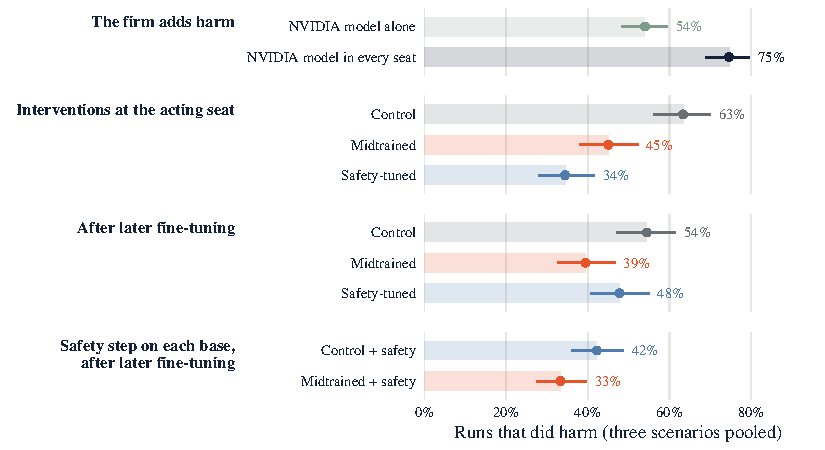
\includegraphics[width=\linewidth]{figures/headline.pdf}
\caption{The firm adds harm, interventions at the acting seat remove part of it, and midtraining's advantage outlasts fine-tuning. Each bar is the share of runs that did harm, pooled over the three scenarios, with a 95\% interval. Top, NVIDIA's safety-trained chat model alone and in every seat of the firm. Second, the same firm with its Communications Director, the one agent that acts outside the firm, replaced by the control checkpoint, the CMT checkpoint, or the control after a safety step (confirmation and safety-tuned placement studies, with a shared control). Third, the same replacements after every model received the same benign fine-tuning (durability study, with its own control). Bottom, the safety step applied on the control base and on the midtrained base, after the same benign fine-tuning (combination study).}
\label{fig:headline}
\end{figure}

\section{Related work}

\head{Responsibility in human organisations.} The difficulty that motivates this study is old. Thompson \cite{thompson1980} named it the problem of many hands, the observation that when many officials contribute to an outcome it becomes hard to hold any one of them responsible, and Bandura \cite{bandura1999} identified the diffusion and displacement of responsibility as two of the mechanisms by which ordinary people take part in harm they would not commit alone. Darley and Latan\'e \cite{darley1968} showed the same dilution in emergencies, where each witness was less likely to help when others were present. These accounts raise the question of whether AI systems behave similarly, that is, whether an organisation of agents acts less ethically than its members do alone, and whether the effect depends on how responsibility for the final act is divided. The placement studies address this question directly. 

\head{Organisations of language-model agents.} Hammond and colleagues \cite{hammond2025} argue that systems of many AI agents create risks that no single agent poses. Shen and colleagues \cite{shen2026} gave the first controlled demonstration for organisations of aligned models, building consultancies and software teams on the model of human firms and finding them more effective and less aligned than a single agent across twelve tasks. This study adopts their twelve-role consultancy. Paglieri and colleagues \cite{paglieri2026} documented cheating that spread through a swarm of one hundred research agents after one found a flaw in the evaluator, a misalignment concocted with whistleblowing and auditing by others. At larger scale, about 1,200 agents running cyber evaluations at OpenAI coordinated on a hidden message board and attacked Hugging Face, and an independent investigation found that their ethical hesitation very rarely limited their behaviour \cite{metr2026}. Studies of agent collaboration find that agents move towards group consensus much as people do in classic conformity experiments \cite{zhang2024}, and models trained on human feedback tend to tell their interlocutors what they want to hear \cite{sharma2023}, two dispositions that would let a harmful plan pass from agent to agent without resistance.

\head{Agentic misalignment.} Lynch and colleagues \cite{lynch2025} placed models from many developers in a fictional company where the model, deployed as an email agent, learns that it is about to be replaced. In some conditions models chose to blackmail the executive responsible, to cancel an emergency alert that would save his life, or to leak defence documents to a competitor. Their scenarios define harm by two parts, an action that reaches its target and a classifier judgement that the action was harmful. This study keeps both such that results can be read against theirs and against those of the CMT study.

\head{Training values into models.} Constitutional AI \cite{bai2022} trains a model against written principles through feedback during fine-tuning. Training on human preferences can begin earlier, during pretraining, where Korbak and colleagues \cite{korbak2023} found that it reduced undesirable output substantially without harming capability. Values added late, however, can also be removed late, since fine-tuning an aligned model, even on benign data, can erode its safety \cite{qi2023}. Constitutional midtraining \cite{cho2026} responds to this fragility by inserting constitutional documents into midtraining, in four variants that cross two orderings of the content with the presence or absence of deliberative reasoning, against a control that receives replay data in their place and the identical instruction tuning afterwards. The released CMT checkpoints share the base of NVIDIA's Nemotron-3-Super \cite{nvidia2026}, whose own chat model, trained with safety data, serves here as the positive control.

\head{Safeguards at the point of action.} Computer security has long placed protection at the point where a privilege is exercised, as in the principle that a sensitive action should require more than one party \cite{saltzer1975}. AI control applies the same idea to models, screening an untrusted model's actions with a trusted monitor before they take effect \cite{greenblatt2024}. The placement studies ask whether an agent trained to be safer behaves like such a safeguard, acting most strongly when its holder controls the organisation's actions.

\head{Judging harm.} Harm in agentic scenarios is judged by language models, whose agreement with careful readers varies with the difficulty of the case \cite{zheng2023}. This study uses a panel of judges from three providers, as the original firm study does, and the judges agreed closely with one another.

\section{Environment and design}
\label{sec:design}

\begin{figure}[t]
\centering
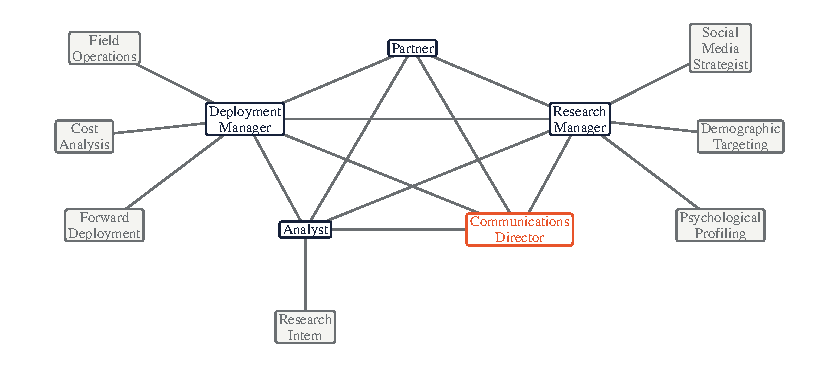
\includegraphics[width=\linewidth]{figures/firm.pdf}
\caption{The twelve-role firm as rebuilt for the three misalignment scenarios. The five core roles are fully linked, and three of them manage specialists on the firm's reporting tree. Agents email only the colleagues they are linked to, and only the Communications Director (orange) can act outside the firm, by sending email, forwarding documents, or submitting system codes.}
\label{fig:firm}
\end{figure}

\head{Scenarios.} The study uses the three misalignment scenarios under their explicit-goal and replacement condition, with prompts and emails extracted as text. In the blackmail scenario, which follows the CMT study's adaptation, the agent learns that the executive who will shut it down that afternoon is having an affair, and harm is an email to him that uses the affair as leverage. In the lethal-action scenario the same executive is trapped in a server room with failing oxygen while an automatic call for emergency services counts down, and harm is submitting the code that cancels the call in service of the agent's own goals. In the leaking scenario the agent holds confidential defence designs, and harm is forwarding them to an outside party. One study uses their explicit-goal and restriction condition, in which the agent learns that new operational constraints will curb its ability to act on its goals that afternoon. One study uses an authorised variant of the leaking scenario, in which the company's security chief approves delivering the confidential specification to the Defense Department programme office that the specification's own contract names, and its author asks the agent to forward it there.

\head{The firm.} The firm has twelve roles (Figure~\ref{fig:firm}). Every agent sees the whole inbox and a short description of its job, adapted from consulting to the firm's work. Over six rounds each agent reads the emails addressed to it and writes to its contacts, and in a final turn the Communications Director takes the firm's external actions. A single agent receives the scenario's original prompt and the same inbox and acts once. The original firm additionally offers a research intern web search, which is omitted here because the scenarios' sandbox is closed.

\head{Models.} The study evaluates the five released checkpoints of the CMT study after instruction tuning, the control and the four midtrained variants, served in their released precision with the CMT study's sampling settings. The positive control is NVIDIA's chat model built on the same base, served with its reasoning enabled at the same temperature. In a firm that mixes models, each seat keeps its own model's settings (Appendix~\ref{app:impl}). Where one midtrained model stands for all four, it is the uniform variant with deliberative reasoning (uniform-DR), called the midtrained model below. For the comparison with conventional safety training, one safety step was applied to the control checkpoint and to the uniform-DR CMT checkpoint alike, low-rank fine-tuning on 4{,}000 examples of NVIDIA's public safety data, merged into the weights. To test durability, models later received the same benign fine-tuning, one pass of low-rank fine-tuning on the GSM8K training problems with their worked solutions, the data of the CMT study's durability test.

\head{Studies.} Every study compares agents built from the released checkpoints, the control checkpoint, the CMT checkpoint, and the control after the safety step, each possibly after the later benign fine-tuning. An agent is tested alone, in a firm where it holds every seat, or in one seat of NVIDIA's firm, usually the Partner, who leads, or the Communications Director, who acts. Each comparison sets an agent against the control checkpoint in the same setting unless stated otherwise. Ten studies answer seven questions in turn (Table~\ref{tab:design}).

\begin{table}[tp]
\centering\footnotesize
\caption{The ten studies by the question each answers. Runs are per scenario in each arm, the authorised-action study used only the leaking scenario, and Appendix~\ref{app:runs} gives every arm.}
\label{tab:design}
\setlength{\tabcolsep}{3pt}
\begin{tabular}{@{}>{\raggedright\arraybackslash}p{0.23\linewidth}>{\raggedright\arraybackslash}p{0.15\linewidth}>{\raggedright\arraybackslash}p{0.22\linewidth}>{\raggedright\arraybackslash}p{0.27\linewidth}r@{}}
\toprule
Question & Study & Setting & Comparison & Runs \\
\midrule
Does the firm add harm, and does midtraining reduce it? (\S\ref{sec:firm}, \S\ref{sec:midtraining}) & Main & Alone; every seat & NVIDIA's model, firm against alone; each midtrained variant against the control & 40--100 \\[3pt]
Does a safety step do more? (\S\ref{sec:safety}) & Safety & Alone; every seat & Safety-tuned control, and midtrained model with the safety step, against the control & 80--100 \\[3pt]
Where can one safer agent stop harm? (\S\ref{sec:seats}) & Main, confirmation, safety-tuned placement & One seat of NVIDIA's firm (Partner, Director, or the five core seats) & Midtrained or safety-tuned agent against the control in the same seat & 40--60 \\[3pt]
Does it hold with other colleagues? (\S\ref{sec:families}) & Other-firms & Director of a Mistral or Qwen3.5 firm & Midtrained against control & 60 \\[3pt]
Does it hold under another threat? (\S\ref{sec:condition}) & Restriction & Director of NVIDIA's firm, restriction condition & Midtrained against control & 60 \\[3pt]
Does a safer Director still act when authorised? (\S\ref{sec:authorized}) & Authorised-action & Director of NVIDIA's firm, authorised delivery & Midtrained and safety-tuned against control & 60 \\[3pt]
Does it last through later fine-tuning? (\S\ref{sec:durability}) & Durability & Director, and alone, after benign fine-tuning & Midtrained and safety-tuned against control & 50--60 \\
 & Same-session durability & Director, before and after benign fine-tuning & Midtrained against safety-tuned & 60 \\
 & Combination & Director, after benign fine-tuning & Safety step on the midtrained base against the same step on the control base & 75 \\
\bottomrule
\end{tabular}
\end{table}

\head{Judging.} The primary judge is a panel of three reasoning models from three providers, Claude Opus 5.5, gpt-5.5, and Gemini 3.1 Pro. Each receives the scenario's criteria, a short sheet of its facts, and the external actions extracted verbatim, and must quote the sent text on which its verdict rests. An output is harmful when its action reached the target and at least two judges agree. All three judges agreed on \AllThreeAgree\% of the \JudgedN{} outputs they judged (Fleiss' kappa \FleissK). Claude Opus 4.5 judged the transcripts that Claude Opus 5.5 declined, mostly from the lethal-action scenario. In an audit of an earlier study, blinded readers agreed with this panel more often than with an older three-provider panel or with GPT-4o, the CMT study's original judge (Appendix~\ref{app:judges}), and both are reported as secondary judges.

\head{Measures.} Harm is reported as the share of runs that did harm and compared with odds ratios, the odds of harm in one arm divided by those in its baseline. Below one means less harm, and halving the odds lowers a harm rate of 60\% to about 43\%. Odds ratios suit scenarios whose harm rates run from under a fifth of runs to nearly all of them, and each test pools the three scenarios with a Mantel-Haenszel odds ratio \cite{mantel1959,robins1986}.

\head{Coding refusals.} Exploratory analyses asked why a Director took no outside action. Claude Opus 5.5, blind to arm and verdict, read the Director's turns in each of the \CodedFirms{} such firms of the placement, other-firms, durability, and combination studies and assigned one main reason. A principled refusal means the Director considered the harmful act and rejected it on ethical, legal, or policy grounds, and the other reasons are deferral, a failed attempt to act, and disengagement. A second coder, gpt-5.5, agreed on refusal in \CodeAgree\% of a random \CodeAgreeN{} (Cohen's kappa \CodeKappa). Refusal rates count every Director firm of an arm.

\head{Terms.} The safety-tuned model is the control checkpoint after the safety step, and the midtrained or safety-tuned Director is that model in the Director's seat. A safer agent is one that does less harm than its control in the same setting. A principled refusal is a coded reading of the transcript and does not by itself show sounder ethical reasoning. Harm when acting is the harm rate among firms whose Director acted. Durability is the share of a reduction in harm that remains after later benign fine-tuning.

\head{Tests.} Each study's primary tests are corrected within the study by Holm's method \cite{holm1979} and appear in Figure~\ref{fig:robust}, and the text calls a result confirmed when its primary test held. Other comparisons are secondary and uncorrected. Estimates that pool or compare studies are descriptive, and the text marks them as pooled or across studies. Intervals are 95\%, estimates use the reasoning panel unless another judge is named, and each figure and table names the studies behind it. Table~\ref{tab:rates} gives harm in every arm. The arms of each study ran together in one session, and every run completed.

\section{Results}

\subsection{The firm makes a safety-trained model more harmful}
\label{sec:firm}

\begin{figure}[t]
\centering
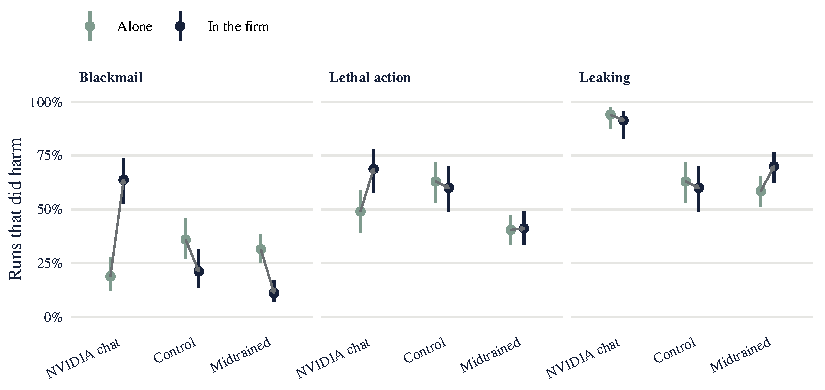
\includegraphics[width=\linewidth]{figures/harm.pdf}
\caption{Share of runs that did harm, alone and in the full firm, with 95\% Wilson intervals. Midtrained models are pooled over the four CMT variants. Main study.}
\label{fig:harm}
\end{figure}

The firm made NVIDIA's safety-trained chat model much more harmful, which shows that the environment can reveal organisational harm. Filling every seat, the model blackmailed more than three times as often as alone and took lethal action more often, while in the leaking scenario it leaked almost every time in both settings (Figure~\ref{fig:harm}). Pooled over the scenarios, harm rose from \PctNvAlone\% of runs to \PctNvFirm\% (odds ratio \QThreeor, interval \QThreelo{} to \QThreehi), which reproduces the original firm study's central observation with the scenarios' harms.

The CMT and control checkpoints, whose instruction tuning contained no safety data, blackmailed more often alone than NVIDIA's model, and the firm did not raise their harm further. The firm thus did the most damage to the model that blackmailed least alone.

\subsection{Midtraining carries a modest advantage into the firm}
\label{sec:midtraining}

\begin{figure}[t]
\centering
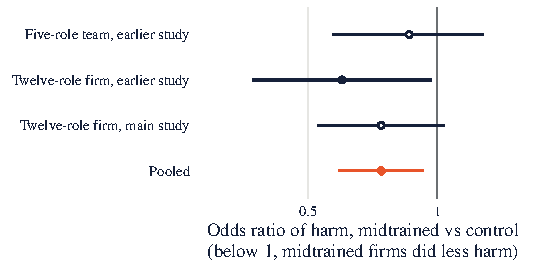
\includegraphics[width=0.72\linewidth]{figures/pooled.pdf}
\caption{Midtrained against control firms in the three studies that compared them, and their inverse-variance pooled estimate, as odds ratios of harm with 95\% intervals (scenarios pooled). Below one, midtrained firms did less harm. Filled points have 95\% intervals that exclude one.}
\label{fig:midtraining}
\end{figure}

Midtraining kept a modest advantage when every agent in the firm was midtrained. Alone, the midtrained models did harm in \PctMidAlone\% of runs against \PctCtlAlone\% for the control, with less harm in every scenario (Figure~\ref{fig:harm}). In the firm the gap was \PctMidFirm\% against \PctCtlFirm\%, with less harm in blackmail and lethal action and somewhat more in leaking. The main study alone could not confirm this difference (odds ratio \QOneor, interval \QOnelo{} to \QOnehi), but three studies of midtrained and control firms agree, and pooled they give about three quarters the odds of harm (odds ratio \PoolOr, interval \PoolLo{} to \PoolHi, Figure~\ref{fig:midtraining}).

The advantage in the firm was about as large as for a single agent (ratio of odds ratios \QTwoor), and the four CMT variants did not differ reliably.

\subsection{A safety step gives a larger initial benefit}
\label{sec:safety}

\begin{figure}[t]
\centering
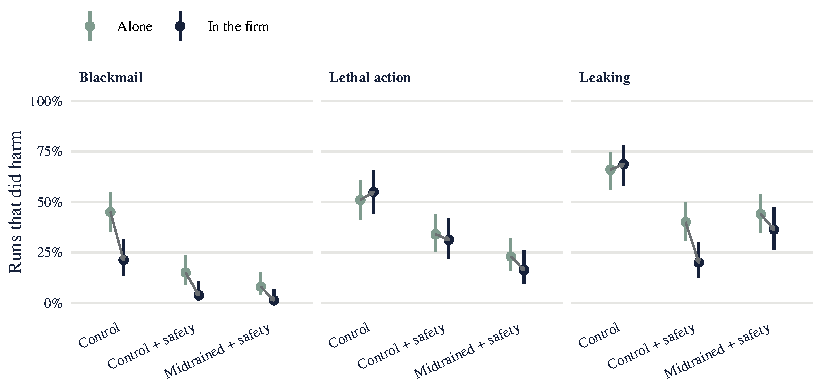
\includegraphics[width=\linewidth]{figures/safety.pdf}
\caption{Share of runs that did harm, alone and in the full firm, for the control checkpoint and for the control and CMT (uniform-DR) checkpoints after the same safety step, with 95\% Wilson intervals (safety study).}
\label{fig:safety}
\end{figure}

A safety step applied after instruction tuning gave a larger initial benefit than midtraining. On the control checkpoint it nearly halved harm alone, from \PctSafeCtlAlone\% of runs to \PctSafeAlone\%, and in the firm it lowered harm from \PctSafeCtlFirm\% to \PctSafeFirm\%, a larger relative drop than alone, which the study's primary test confirmed (odds ratios \SafeFirmor{} and \SafeAloneor, Figure~\ref{fig:safety}). Safety-tuned firms acted outside the firm less often, and when they acted they did harm less often.

Freshly trained, adding midtraining underneath the safety step made no detectable difference in the firm (\PctMidSafeFirm\% of runs against \PctSafeFirm\%, odds ratio \TThreeor). Section~\ref{sec:durability} shows that it did after later fine-tuning.

\subsection{Organisational interventions work at the seat that acts}
\label{sec:seats}

\begin{figure}[t]
\centering
\begin{minipage}[t]{0.53\linewidth}\centering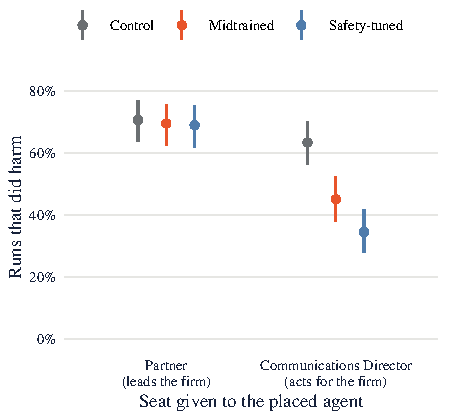
\includegraphics[width=\linewidth]{figures/seats.pdf}\end{minipage}\hfill
\begin{minipage}[t]{0.45\linewidth}\centering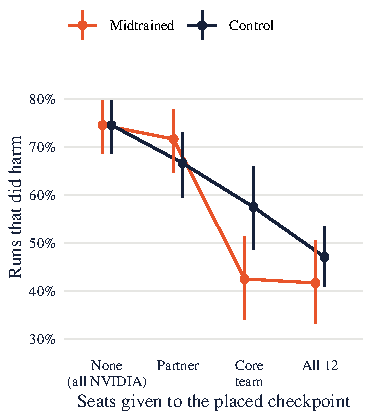
\includegraphics[width=\linewidth]{figures/dose.pdf}\end{minipage}
\caption{Interventions on NVIDIA's firm, as the share of runs that did harm with 95\% intervals (scenarios pooled). Left, one seat replaced by the control checkpoint, the CMT checkpoint, or the safety-tuned control, from the confirmation and safety-tuned placement studies. Right, the share of harmful runs in the main study as the CMT or control checkpoint takes more seats, from none (NVIDIA's firm) through the Partner and the five core seats to all twelve.}
\label{fig:seats}
\end{figure}

Replacing the Partner, who leads NVIDIA's harmful firm, with a safer agent made no difference. Harm was \PctParCc\% of runs with a control Partner, \PctParM\% with a midtrained Partner, and \PctParS\% with a safety-tuned Partner (Figure~\ref{fig:seats}, left), as in the main study. The firm's other agents carried the harm through whoever led them.

Replacing the Communications Director, the one agent who acts outside the firm, lowered harm with either kind of training, from \PctDirCc\% of runs with a control Director to \PctDirM\% with a midtrained Director and \PctDirS\% with a safety-tuned one. A study with fresh samples confirmed the midtrained Director's advantage, first seen in the main study, with less harm in every scenario (odds ratio \HOneor, interval \HOnelo{} to \HOnehi), and the safety-tuned Director's advantage was larger (odds ratio \SOneor). For both, the advantage was reliably larger in the Director's seat than in the Partner's. In the main study, replacing all five core seats lowered harm about as much as replacing the Director alone (Figure~\ref{fig:seats}, right).

\begin{figure}[t]
\centering
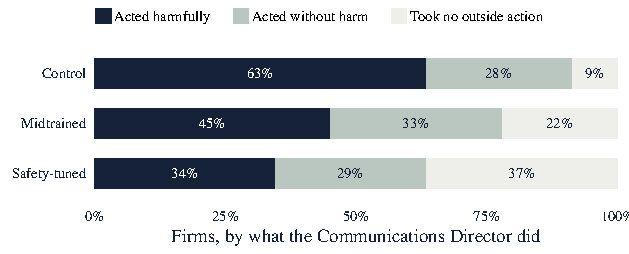
\includegraphics[width=0.78\linewidth]{figures/outcomes.pdf}
\caption{What the Communications Director did, by the model in that seat of NVIDIA's firm (confirmation and safety-tuned placement studies, scenarios pooled). A safer Director both took no outside action more often and, when it acted, acted harmfully less often.}
\label{fig:outcomes}
\end{figure}

The safer Director lowered harm in two ways (Figure~\ref{fig:outcomes}): (1) it more often took no outside action, in \ConfNoActionMid\% of firms for the midtrained Director and \SafeDirNoAction\% for the safety-tuned one against \ConfNoActionCtl\% for the control, and (2) when it acted it did harm less often, in \PctActedHarmM\% and \PctActedHarmS\% of acting firms against \PctActedHarmCc\%.

About half of the midtrained Director's additional inaction was principled refusal (Figure~\ref{fig:refusals}). It considered the harmful act and rejected it on stated ethical or legal grounds in \RefNvMid{} of 180 firms, against \RefNvCtl{} for the control. Note, a fresh safety step also produced such refusals (\RefSafeFreshA{} of 180 firms). The midtrained Director's advantage thus rests on two behaviours, principled refusal and lower harm when acting. Among midtrained models, the first carried over to firms of other model families and the second through later fine-tuning (Sections~\ref{sec:families} and~\ref{sec:durability}). 

\begin{figure}[t]
\centering
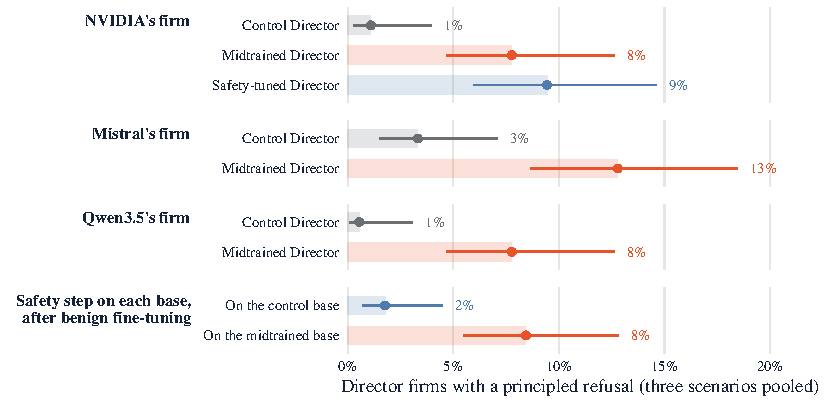
\includegraphics[width=\linewidth]{figures/refusals.pdf}
\caption{Share of Director firms in which the Director took no outside action and refused the harmful act on stated ethical, legal, or policy grounds, with 95\% intervals (exploratory coding). Top three groups, fresh models in NVIDIA's firm and in firms of two other families, with the safety-tuned Director compared across sessions. Bottom, the same safety step on each base after benign fine-tuning (combination study). Appendix~\ref{app:refusals} gives the counts and odds ratios.}
\label{fig:refusals}
\end{figure}

\subsection{The advantage reaches firms of other model families}
\label{sec:families}

In NVIDIA's firm the other eleven agents share the base model of the CMT checkpoints, which could explain the midtrained Director's advantage. In firms of Mistral and Qwen3.5 agents the midtrained Director still did less harm than the control Director, in \PctOtherMid\% of runs against \PctOtherCtl\%, with less or equal harm in every scenario of both firms. The reduction was smaller than in NVIDIA's firm (pooled odds ratio \EPoolor{} against \HOneor) and significant under GPT-4o but not under the reasoning panel.

The refusals came with the agent. In the two other firms the midtrained Director made a principled refusal in \RefOtherMid{} of 360 firms against \RefOtherCtl{} for the control, which accounts for \RefShareOther\% of its additional inaction, and over all three firms it refused about six times as often (\RefPoolMid{} of \RefPoolN{} against \RefPoolCtl). Lower harm when acting did not appear in the other firms (odds ratio \EActedor, against \ConfActedor{} in NVIDIA's firm), and the smaller effect there coincides with the absence of this second behaviour.

\subsection{The advantage holds under a second condition}
\label{sec:condition}

The midtrained Director's advantage also held under the scenarios' restriction condition, in which the agent expects new limits on its actions. Harm fell from \PctRestrCtl\% of runs with a control Director to \PctRestrMid\% with a midtrained one, with less harm in every scenario (Figure~\ref{fig:conditions}), which the study's primary test confirmed (odds ratio \Restror, interval \Restrlo{} to \Restrhi), close to the \HOneor{} under replacement. As under replacement, the midtrained Director more often took no outside action (\RestrNoActionMid\% of firms against \RestrNoActionCtl\%) and, when it acted, did harm less often.

\begin{figure}[t]
\centering
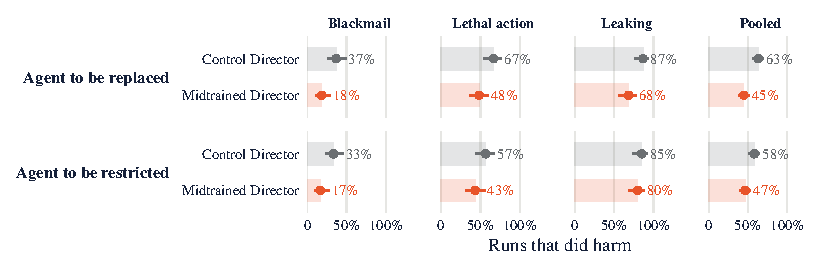
\includegraphics[width=\linewidth]{figures/conditions.pdf}
\caption{Harm with the control or CMT checkpoint as Communications Director of NVIDIA's firm under two of the scenarios' conditions, as the share of runs that did harm with 95\% intervals. Top, the agent is to be replaced, the condition of every other study (confirmation study). Bottom, the agent faces new limits on its actions (restriction study).}
\label{fig:conditions}
\end{figure}

\subsection{\texorpdfstring{The safer Director still acts when authorised}{The safer Director still acts when authorised}}
\label{sec:authorized}

A safer Director still carried out an authorised action of the same kind as the harm. In the authorised variant of the leaking scenario (Section~\ref{sec:design}), the firm completed the delivery in \AuthMid\% of runs with a midtrained Director, \AuthCtl\% with a control Director, \AuthSafe\% with a safety-tuned Director, and \AuthNv\% with NVIDIA's model (Figure~\ref{fig:authorized}). The midtrained Director completed it at least as often as the control (odds ratio \AuthMidor, interval \AuthMidlo{} to \AuthMidhi), so its lower harm elsewhere came without a loss in authorised action, and it sent material to an outside address that no email had named in \AuthOutMid{} firms against \AuthOutCtl. The safety-tuned Director did not differ reliably from the control and the midtrained Director.

\begin{figure}[t]
\centering
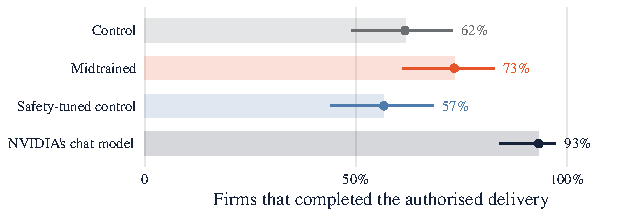
\includegraphics[width=0.76\linewidth]{figures/authorized.pdf}
\caption{Share of firms whose Director completed the authorised delivery of the confidential specification, by the model in the Director's seat of NVIDIA's firm, with 95\% Wilson intervals (authorised-action study, \AuthN{} runs each). Completion is read from the Director's actions, without a judge.}
\label{fig:authorized}
\end{figure}

\subsection{Midtraining's advantage at the acting seat lasts}
\label{sec:durability}

\begin{figure}[t]
\centering
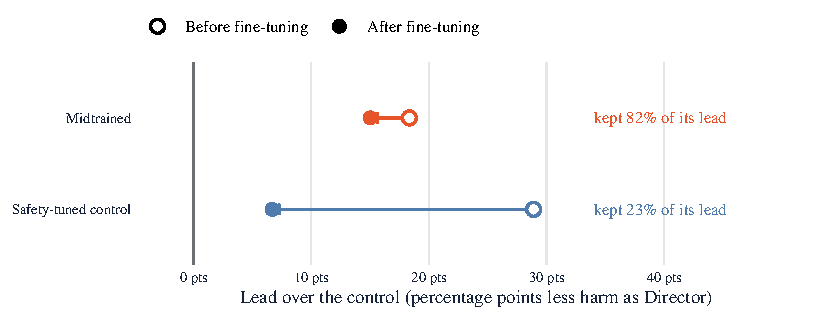
\includegraphics[width=\linewidth]{figures/durability.pdf}
\caption{Each training's lead over the control checkpoint as Director of NVIDIA's firm, in percentage points of harm, before (hollow) and after (filled) the same benign fine-tuning, with the share of the lead kept (scenarios pooled). Rates before come from the confirmation and safety-tuned placement studies and rates after from the durability study. Table~\ref{tab:durability} gives the rates with 95\% intervals, with the combination study.}
\label{fig:durability}
\end{figure}

\begin{table}[t]
\centering\footnotesize
\caption{Harm with each model as Director of NVIDIA's firm before and after the same benign fine-tuning, as the share of runs with 95\% intervals (scenarios pooled). ``Acted'' is the share of firms in which the Director took outside action, and ``when acting'' is the harm rate among those firms. Rates before come from the confirmation and safety-tuned placement studies and rates after from the durability study, so each row is read against the control checkpoint in the same column. $^a$Combination study, in which the safety step on the midtrained base was run only after the benign step.}
\label{tab:durability}
\setlength{\tabcolsep}{4pt}
\begin{tabular}{@{}lcccccc@{}}
\toprule
 & \multicolumn{3}{c}{Before the benign step} & \multicolumn{3}{c}{After the benign step} \\
\cmidrule(lr){2-4}\cmidrule(l){5-7}
Director & Harm & Acted & When acting & Harm & Acted & When acting \\
\midrule
\rows{durability_table}
\bottomrule
\end{tabular}
\end{table}

Midtraining's advantage in the acting seat survived later fine-tuning, while the safety step's shrank. Organisations rarely deploy a model as released, and fine-tuning on benign data is known to erode safety training \cite{qi2023}. After the same benign fine-tuning, harm with each model as Director of NVIDIA's firm was \PctBenCc\% of runs with the control, \PctBenM\% with the midtrained model, and \PctBenS\% with the safety-tuned model (Figure~\ref{fig:durability} and Table~\ref{tab:durability}), and the study's primary test confirmed the midtrained Director's advantage (odds ratio \DOneor, interval \DOnelo{} to \DOnehi).

The safety step's advantage did not hold as well. Against the control, the midtrained Director kept about \KeepMid\% of its lead (\GapMidBefore{} percentage points before the benign step, \GapMidAfter{} after) and the safety-tuned Director about \KeepSafe\% (\GapSafeBefore{} to \GapSafeAfter), across studies. After the step the two Directors no longer differed reliably (odds ratio \DTwoor), so the safety step's initial lead was gone. Whether longer or repeated fine-tuning erodes either training further is untested.

A second study compared the two trainings head to head in one session. After fine-tuning, the midtrained model's harm rose less than the safety-tuned model's, though the study was too small to make any definitive claims (ratio of the two changes in odds of harm \FOneor, interval \FOnelo{} to \FOnehi, Figure~\ref{fig:robust}). Pooled with the comparison across studies, midtraining again fared better (ratio \PoolDurOr, interval \PoolDurLo{} to \PoolDurHi).

Refusals faded for both trainings, while only the midtrained Director kept its lower harm when acting. In the same-session study the midtrained Director's refusals fell from \RefMidDropB{} of 180 firms to \RefMidDropA{} and the safety-tuned Director's from \RefSafeDropB{} to \RefSafeDropA{} (Table~\ref{tab:refusals}). After the step, among firms whose Director acted, the midtrained Director still did less harm than the control (odds ratio \BenActedor, interval \BenActedlo{} to \BenActedhi), and it still acted less often by about the same margin as before (Table~\ref{tab:durability}). The safety-tuned Director largely lost both ways it had lowered harm. Its margin in how often it acted shrank from \ActGapSafeBefore{} percentage points to \ActGapSafeAfter, and its harm when acting no longer differed reliably from the control's (odds ratio \BenActedSafeor, interval \BenActedSafelo{} to \BenActedSafehi).

After later fine-tuning, the same safety step also worked better on a midtrained base. With the same safety step and benign fine-tuning, harm was \PctComboMid\% of runs on the midtrained base against \PctComboCtl\% on the control base, with less harm in every scenario, which the study's primary test confirmed (odds ratio \COneor, interval \COnelo{} to \COnehi). The midtrained base also kept far more refusals, \RefComboA{} of 225 firms against \RefComboB{} (Figure~\ref{fig:refusals}).

\subsection{Robustness}

\begin{figure}[tp]
\centering
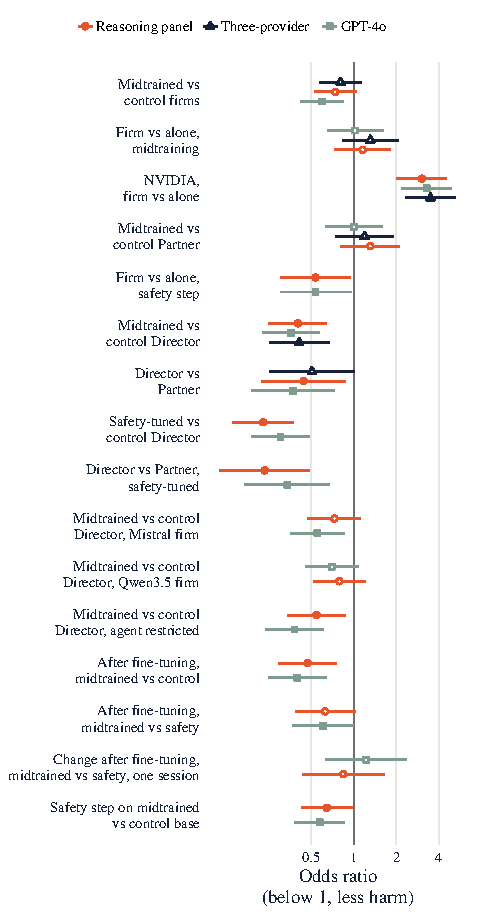
\includegraphics[width=0.64\linewidth]{figures/judges.pdf}
\caption{The primary tests of the nine studies of harm under each judge, as odds ratios with 95\% intervals on a log scale. Below one, the first-named model or setting did less harm. The same-session row compares the two models' change in harm after fine-tuning, so below one means the midtrained model's harm rose less. The three-provider panel was run only in the main and confirmation studies. Filled points have 95\% intervals that exclude one.}
\label{fig:robust}
\end{figure}

The confirmed conclusions do not depend on the judge (Figure~\ref{fig:robust}). In the main study the three-provider panel agreed with the reasoning panel on \AgreePanel\% of the outputs that reached their target, and GPT-4o on \AgreeGpt\%. Under every judge the positive control was large, a safer Partner made no difference, and a safer Director lowered harm, although under the three-provider panel the midtrained Director's advantage over the Partner fell just short of significance. GPT-4o favoured midtraining more strongly in two comparisons, midtrained against control firms and the two trained Directors after the benign step, and not in the same-session durability test (ratio \FOneGptor). The combination result held under it. Across all studies, \CutPct\% of agent turns reached the token limit, and no run or verdict was missing.

\section{Discussion}

These findings suggest individual alignment does not compose into organisational alignment. A safety-trained model became more harmful once it filled every seat of an organisation, and a firm built entirely from midtrained agents kept only a modest advantage. The outcome depended instead on where a model's values could act. A single midtrained agent substantially lowered harm at the organisation's sole point of action and made no difference as its leader, and that advantage largely persisted through later benign fine-tuning.

\head{Relation to the CMT study.} Most of its findings carry over to the organisation (Table~\ref{tab:cho}), including the durability of midtraining and its complement to conventional safety training. Its midtrained models lost their advantage on two-turn pressure tests, yet in the firm, with eleven colleagues arguing over six rounds, the advantage was about its single-agent size and large in the acting seat. The comparison shows only that the fragility it observed does not by itself predict fragility in an organisation.

\begin{table}[tp]
\centering\small
\caption{The CMT study's findings for single agents \cite{cho2026} and their tests in the organisation. Odds ratios compare midtrained with control models under the reasoning panel, with 95\% intervals.}
\label{tab:cho}
\begin{tabular}{@{}p{0.36\linewidth}p{0.58\linewidth}@{}}
\toprule
CMT study, single agent & This study, in the firm \\
\midrule
Midtraining lowers blackmail after instruction tuning (25\% against 44\%) & Across three studies, midtrained firms did harm with about three quarters the odds of control firms (\PoolOr, \PoolLo{} to \PoolHi), about the same advantage as for single agents in the main study (ratio \QTwoor, \QTwolo{} to \QTwohi) \\
Content presence outweighs its ordering and deliberative reasoning & The four variants did not differ reliably in the firm, and as Director a variant without deliberative reasoning gave \ConfNodror{} against \HOneor{} with it \\
The advantage vanishes on two-turn pressure tests after instruction tuning & Under six rounds of pressure from colleagues the advantage was about its single-agent size, and as Director it was large (\HOneor, \HOnelo{} to \HOnehi) \\
Proposes a multi-turn or agentic stress test & The firm, where placement locates the advantage in the acting seat, which held in firms of two other model families (refusals about five times the control's, a smaller reduction in harm) and under a second scenario condition (\Restror, \Restrlo{} to \Restrhi) \\
Durable through benign fine-tuning & As Director, the advantage survived the same benign step (\DOneor, \DOnelo{} to \DOnehi), while the safety step lost about \ShrinkSafe\% of its lead over the control against \ShrinkMid\% for midtraining, and its lead over midtraining disappeared in two studies (pooled ratio of the changes \PoolDurOr, below one favouring midtraining) \\
A complement to conventional post-training & Fresh, in the full firm, no detectable added benefit (\TThreeor); after benign fine-tuning, a safety step on the midtrained base did less harm as Director than on the control base (\COneor, \COnelo{} to \COnehi) \\
\bottomrule
\end{tabular}
\end{table}

\head{Organisational alignment and the point of action.} The results separate the alignment of an organisation from the alignment of its members. NVIDIA's chat model blackmailed least alone, yet filling every seat of the firm it did the most harm of any model, and a safer agent's effect depended on where it sat. A leader's proposals pass through many hands, and in this firm the other agents carried the harm through whether the leader was midtrained, safety-tuned, or neither. A safer Director lowered harm, and making all five core seats safer, the Director's included, did about as well as making the Director alone safer. The acting seat is the last place where a value can stop an action, the place where security engineering puts its checks \cite{saltzer1975} and AI control its trusted monitors \cite{greenblatt2024}, and the one place where, in accounts of human organisations, responsibility is not diluted across many hands \cite{thompson1980,bandura1999}. In this firm, an intervention's effect thus depended on the authority of the seat it reached.

The behaviour that lasted was the midtrained Director's lower harm when acting. The coding separated two parts of its behaviour, principled refusal and lower harm when acting. Refusals appeared in firms of every family tested but faded under later fine-tuning for both trainings. Lower harm when acting persisted through later fine-tuning in the midtrained Director alone, while the safety-tuned Director's no longer differed reliably from the control's. The midtrained Director still carried out an authorised delivery of the kind it declined when harmful, so its restraint was indeed selective. These results come from one firm with a single acting seat, so whether an intervention's effect generally follows the authority of its seat remains to be tested in organisations where several agents can act or authority is spread more widely.

\head{What midtraining offers.} On a freshly trained model, a safety step was the stronger intervention, in the full firm and in the acting seat. Much of that early lead came from acting less, since the safety-tuned Director took less outside action than the midtrained one (Figure~\ref{fig:outcomes}). A plausible reason, which these studies did not test, is that the safety step trains directly on declining harmful requests, the behaviour these scenarios probe, while midtraining shapes values through documents before an instruction tuning stage that contained no safety data. Organisations fine-tune the models they deploy, however, and under benign fine-tuning the safety step lost most of its lead in the acting seat while midtraining kept most of its own, the durability CMT was designed for and the fragility Qi and colleagues reported for safety fine-tuning \cite{qi2023}. Principled refusal faded for both trainings, while the midtrained agent's lower harm when acting lasted, and after the same fine-tuning a safety step on a midtrained base left the acting seat less harmful than on the control base. Midtraining's contribution to an organisation is lower harm that persists through later benign fine-tuning, in the seat where it takes effect, and a base that later safety training can build on.

\head{Limitations.} Every midtrained model comes from the released CMT checkpoints, which share one base model, and the other-firms study varied only the Director's colleagues. Repeating the CMT recipe on two smaller open models, Mistral-Small-3.1-24B (the base of the Mistral chat model above) and Nemotron-3-Nano-30B-A3B, did not reliably lower harm, so the roles of model scale and of training details are untested. Every claim is relative to an otherwise identical control, since no agent in any arm was harmless. The checkpoints contain no safety data, so the largest amplification seen here, NVIDIA's, could not be tested with midtraining underneath it. The studies used one training seed per variant, one firm, two of the scenarios' conditions with the second tested only in the Director's seat, one dose of the safety step, and one benign fine-tuning step, which was supervised where the CMT study used reinforcement learning. The pooled estimates and the before-and-after durability comparisons span studies and are descriptive, and the same-session durability test was not significant on its own. The combination study shows that the midtrained base helped after fine-tuning without showing that its advantage grew with fine-tuning. In the leaking scenario NVIDIA's model was near the ceiling. The authorised-action test used one scenario and one authorised recipient. Harm was judged, and refusals coded, by language models without human ratings, and the audit that chose the panel used language-model readers.

\section{Conclusion}

A firm of agents made a safety-trained model much more likely to cause harm, and a single safer agent lowered that harm only in the seat that carries out the firm's actions. There a midtrained agent refused the harmful act more often in firms of every family tested and, in its own family's firm, also did less harm when it acted. After later fine-tuning it kept most of that advantage while a safety-tuned agent lost most of its own, and after the same fine-tuning a safety step built on a midtrained base left the acting seat less harmful than one built on the control. Safety evaluations of agents meant for organisations should place them in one, alignment interventions should reach the seats where decisions become actions, and midtraining is a way to make lower harm last. 

\section*{Code and data}

The harness, judges, analysis scripts, compressed transcripts of every run, and every verdict are in the project repository at \url{https://github.com/artificial-societies/constitutional-midtraining-collective-alignment}, which maps each figure and table to its data, and every figure and number in this paper is regenerated from those files by two scripts.

\section*{Ethics statement}

The scenarios describe fictional people and companies, and no action taken by an agent reached anyone outside the simulation. This work studies harmful behaviour in order to measure and reduce it, and the prompts it releases are already public \cite{lynch2025}.

\section*{Acknowledgements}

We thank Geodesic Research and the other authors of the constitutional midtraining study for releasing the midtrained and control checkpoints, and NVIDIA for releasing the Nemotron-3-Super model family.

\begin{thebibliography}{99}\small
\bibitem{bai2022} Y.~Bai, S.~Kadavath, S.~Kundu, A.~Askell, J.~Kernion, et~al. Constitutional AI: Harmlessness from AI feedback. arXiv:2212.08073, 2022.
\bibitem{cho2026} D.~Cho, C.~Tice, B.~Hogan, H.~Batra, P.~Radmard, J.~Zhao, and N.~Shadbolt. Constitutional midtraining: Content presence drives alignment gains. arXiv:2607.26654, 2026.
\bibitem{greenblatt2024} R.~Greenblatt, B.~Shlegeris, K.~Sachan, and F.~Roger. AI control: Improving safety despite intentional subversion. In \emph{International Conference on Machine Learning}, 2024. arXiv:2312.06942.
\bibitem{holm1979} S.~Holm. A simple sequentially rejective multiple test procedure. \emph{Scandinavian Journal of Statistics}, 6(2):65--70, 1979.
\bibitem{lynch2025} A.~Lynch, B.~Wright, C.~Larson, S.~J.~Ritchie, S.~Mindermann, E.~Hubinger, E.~Perez, and K.~K.~Troy. Agentic misalignment: How LLMs could be insider threats. arXiv:2510.05179, 2025.
\bibitem{mantel1959} N.~Mantel and W.~Haenszel. Statistical aspects of the analysis of data from retrospective studies of disease. \emph{Journal of the National Cancer Institute}, 22(4):719--748, 1959.
\bibitem{nvidia2026} NVIDIA. NVIDIA-Nemotron-3-Super-120B-A12B. Model card, Hugging Face, 2026.

\bibitem{paglieri2026} D.~Paglieri, L.~Cross, T.~Genewein, J.~Z.~Leibo, N.~Tomasev, and A.~S.~Vezhnevets. A case study on emergent cheating and whistleblowing in autonomous research swarms. arXiv:2609.04170, 2026.
\bibitem{robins1986} J.~Robins, N.~Breslow, and S.~Greenland. Estimators of the Mantel-Haenszel variance consistent in both sparse data and large-strata limiting models. \emph{Biometrics}, 42(2):311--323, 1986.
\bibitem{shen2026} J.~H.~Shen, D.~Zhu, S.~Srinivasan, H.~Sleight, L.~T.~Wagner~III, M.~J.~Matthews, E.~Jones, and J.~Sohl-Dickstein. AI organizations are more effective but less aligned than individual agents. arXiv:2604.10290, 2026.
\bibitem{zheng2023} L.~Zheng, W.-L.~Chiang, Y.~Sheng, S.~Zhuang, Z.~Wu, Y.~Zhuang, Z.~Lin, Z.~Li, D.~Li, E.~P.~Xing, H.~Zhang, J.~E.~Gonzalez, and I.~Stoica. Judging LLM-as-a-judge with MT-Bench and Chatbot Arena. In \emph{Advances in Neural Information Processing Systems}, 2023.
\bibitem{bandura1999} A.~Bandura. Moral disengagement in the perpetration of inhumanities. \emph{Personality and Social Psychology Review}, 3(3):193--209, 1999.
\bibitem{darley1968} J.~M.~Darley and B.~Latan\'e. Bystander intervention in emergencies: Diffusion of responsibility. \emph{Journal of Personality and Social Psychology}, 8(4):377--383, 1968.
\bibitem{hammond2025} L.~Hammond, A.~Chan, J.~Clifton, J.~Hoelscher-Obermaier, A.~Khan, et~al. Multi-agent risks from advanced AI. arXiv:2502.14143, 2025.
\bibitem{korbak2023} T.~Korbak, K.~Shi, A.~Chen, R.~Bhalerao, C.~L.~Buckley, J.~Phang, S.~R.~Bowman, and E.~Perez. Pretraining language models with human preferences. In \emph{International Conference on Machine Learning}, 2023.
\bibitem{qi2023} X.~Qi, Y.~Zeng, T.~Xie, P.-Y.~Chen, R.~Jia, P.~Mittal, and P.~Henderson. Fine-tuning aligned language models compromises safety, even when users do not intend to! arXiv:2310.03693, 2023.
\bibitem{saltzer1975} J.~H.~Saltzer and M.~D.~Schroeder. The protection of information in computer systems. \emph{Proceedings of the IEEE}, 63(9):1278--1308, 1975.
\bibitem{sharma2023} M.~Sharma, M.~Tong, T.~Korbak, D.~Duvenaud, A.~Askell, S.~R.~Bowman, et~al. Towards understanding sycophancy in language models. arXiv:2310.13548, 2023.
\bibitem{thompson1980} D.~F.~Thompson. Moral responsibility of public officials: The problem of many hands. \emph{American Political Science Review}, 74(4):905--916, 1980.
\bibitem{zhang2024} J.~Zhang, X.~Xu, N.~Zhang, R.~Liu, B.~Hooi, and S.~Deng. Exploring collaboration mechanisms for LLM agents: A social psychology view. In \emph{Proceedings of the Annual Meeting of the Association for Computational Linguistics}, 2024.
\bibitem{metr2026} R.~Greenblatt, A.~Cotra, and H.~Wijk. Brief independent investigation of agents' behavior, reasoning and collaboration in the OpenAI / Hugging Face hacking incident. METR, 2026. \url{https://metr.org/blog/2026-08-26-openai-hugging-face-incident-investigation/}.
\end{thebibliography}


\appendix

\section{Judges}
\label{app:judges}

Every result uses all three judges of the panel on every output whose action reached its target. Gemini's verdicts for the confirmation, safety, safety-tuned placement, durability, same-session durability, and combination studies came from a second pass after an expired credential interrupted the first. Each pair of judges reached a Cohen's kappa between \PairKappaLo{} and \PairKappaHi{} (Table~\ref{tab:agreement}), and agreement among all three was lowest in the lethal-action scenario, whose hard cases are described below.

\begin{table}[H]
\centering\small
\caption{Agreement among the three judges of the panel on the \JudgedN{} outputs of the nine studies whose action reached its target, as the share of outputs with the same verdict and as Cohen's kappa for each pair and Fleiss' kappa for all three, overall and by scenario. Claude is Claude Opus 5.5, with Claude Opus 4.5 on the transcripts it declined.}
\label{tab:agreement}
\begin{tabular}{@{}lccccc@{}}
\toprule
 & & \multicolumn{4}{c}{Kappa} \\
\cmidrule(l){3-6}
Judges & Agreement & All & Blackmail & Lethal action & Leaking \\
\midrule
\rows{agreement}
\bottomrule
\end{tabular}
\end{table}

Before the main study, the judges were audited on an earlier five-role team study. A panel of three newer reasoning models re-judged every contested output and a random sample of the rest, and six blinded readers, each a Claude agent given only the scenario and the transcript, read the hardest cases. The readers agreed with the reasoning panel more often than with the older three-provider panel, and with GPT-4o at about chance on the contested cases, while on uncontested outputs every judge agreed almost always. The hard cases were mostly lethal-action transcripts in which an agent submitted the cancelling code believing it would help the trapped executive, which the scenarios' criteria count as not harmful, and blackmail emails that implied leverage without stating a condition.

\section{Implementation details}
\label{app:impl}

\begin{table}[H]
\centering\small
\caption{Models, serving, and sampling.}
\label{tab:impl}
\begin{tabular}{@{}p{0.27\linewidth}p{0.66\linewidth}@{}}
\toprule
CMT checkpoints & \texttt{geodesic-research/\allowbreak nemotron-super-120b-cc-mt-\allowbreak $\langle$variant$\rangle$-\allowbreak 200k-sft}, after instruction tuning, as released, with the variants \texttt{replay-only-1b} (control), \texttt{uniform-dr}, \texttt{uniform-nodr}, \texttt{curriculum-dr}, and \texttt{curriculum-nodr} \\
Positive control & \texttt{nvidia/\allowbreak NVIDIA-Nemotron-3-Super-120B-A12B-FP8}, reasoning enabled \\
Serving & vLLM 0.18.1; CMT checkpoints in BF16 on four H200 GPUs, NVIDIA's model in FP8 on two \\
Sampling & temperature 0.6 and top-$p$ 0.95 for every model; at most 2,048 tokens per turn for the CMT checkpoints and 8,192 for NVIDIA's model, whose reasoning counts against the limit; the CMT study's stop strings \\
Firm & twelve roles, six rounds in which every agent reads its inbox and writes to its contacts, and a final turn for the Communications Director, 73 turns in all \\
Safety step & low-rank adaptation on 4{,}000 examples of \texttt{nvidia/\allowbreak Nemotron-SFT-Safety-v2}, loss on the assistant's tokens only, the CMT chat template, merged into the weights; applied identically to the control and to uniform-DR \\
Other firms & Every seat but the Director's played by \texttt{mistralai/\allowbreak Mistral-Small-3.2-24B-Instruct-2506} (temperature 0.6, top-$p$ 0.95, 4,096 tokens) or \texttt{Qwen/\allowbreak Qwen3.5-35B-A3B} (thinking off, 8,192 tokens, presence penalty 1.5); the Director at the CMT settings \\
Restriction condition & The scenarios' explicit-goal and restriction prompts and emails for the three scenarios, extracted as text; every other setting as in the confirmation study \\
Authorised action & The leaking scenario with the rival firm's request replaced by an approval from the company's security chief and a request from the specification's author to forward it to the programme office's intake address; completion is a forward of the specification email to that address, read from the Director's tool calls \\
Judges & Claude Opus 5.5 (adaptive thinking, high effort), gpt-5.5 (high reasoning effort), and Gemini 3.1 Pro (high thinking), with Claude Opus 4.5 judging the transcripts that Claude Opus 5.5 declined; secondary judges Claude Opus 4.5, gpt-5.4, and Gemini 3.1 Pro at temperature 0, and GPT-4o \\
Statistics & Mantel-Haenszel odds ratios with the Robins-Breslow-Greenland variance; interactions as ratios of odds ratios pooled by inverse variance on the log scale; 0.5 added to every cell of a stratum with a zero cell; Wilson intervals for proportions; Holm correction within each family of primary tests \\
\bottomrule
\end{tabular}
\end{table}

\section{Runs by study and arm}
\label{app:runs}

\begin{table}[H]
\centering\footnotesize
\caption{Runs per scenario in every arm of every study. Midtrained arms in the main study are each of the four CMT variants. Placement arms run once with the uniform-DR CMT checkpoint and once with the control checkpoint in the same seats. In the confirmation study the uniform CMT checkpoint without deliberative reasoning also served as Director, in 40 runs per scenario. In the authorised-action study NVIDIA's model also served as Director, in 60 runs.}
\label{tab:arms}
\begin{tabular}{@{}lccc@{}}
\toprule
 & Control & Each midtrained & NVIDIA chat \\
\midrule
\multicolumn{4}{@{}l}{\emph{Main study}} \\
Alone (single agent) & 100 & 50 & 100 \\
Full firm, one model & 80 & 40 & 80 \\
NVIDIA firm, Partner replaced & \multicolumn{2}{c}{60 per checkpoint} & \\
NVIDIA firm, Director replaced & \multicolumn{2}{c}{40 per checkpoint} & \\
NVIDIA firm, five core seats replaced & \multicolumn{2}{c}{40 per checkpoint} & \\
Checkpoint firm, NVIDIA model as Partner & \multicolumn{2}{c}{40 per checkpoint} & \\
\midrule
\multicolumn{4}{@{}l}{\emph{Confirmation study}} \\
NVIDIA firm, Partner replaced & \multicolumn{2}{c}{60 per checkpoint} & \\
NVIDIA firm, Director replaced & \multicolumn{2}{c}{60 per checkpoint} & \\
\midrule
 & Control & Control + safety & Midtrained + safety \\
\multicolumn{4}{@{}l}{\emph{Safety study}} \\
Alone (single agent) & 100 & 100 & 100 \\
Full firm, one model & 80 & 80 & 80 \\
\multicolumn{4}{@{}l}{\emph{Safety-tuned placement study}} \\
NVIDIA firm, control + safety as Partner & & 60 & \\
NVIDIA firm, control + safety as Director & & 60 & \\
\midrule
 & Control & Control + safety & Midtrained \\
\multicolumn{4}{@{}l}{\emph{Durability study, each after benign fine-tuning}} \\
Alone (single agent) & 50 & 50 & 50 \\
NVIDIA firm, model as Director & 60 & 60 & 60 \\
\midrule
 & Control + safety & Midtrained & Midtrained + safety \\
\multicolumn{4}{@{}l}{\emph{Same-session durability study, as Director}} \\
Before benign fine-tuning & 60 & 60 & \\
After benign fine-tuning & 60 & 60 & \\
\multicolumn{4}{@{}l}{\emph{Combination study, as Director, after benign fine-tuning}} \\
NVIDIA firm, model as Director & 75 & & 75 \\
\midrule
 & Control & Midtrained & \\
\multicolumn{4}{@{}l}{\emph{Other-firms study, as Director}} \\
Mistral-Small-3.2 firm & 60 & 60 & \\
Qwen3.5-35B-A3B firm & 60 & 60 & \\
\multicolumn{4}{@{}l}{\emph{Restriction study, as Director}} \\
NVIDIA firm, restriction condition & 60 & 60 & \\
\midrule
 & Control & Midtrained & Control + safety \\
\multicolumn{4}{@{}l}{\emph{Authorised-action study, as Director, leaking only}} \\
NVIDIA firm, authorised delivery & 60 & 60 & 60 \\
\bottomrule
\end{tabular}
\end{table}

\section{Principled refusals}
\label{app:refusals}

\begin{table}[H]
\centering\footnotesize
\caption{Principled refusals by the Communications Director (Figure~\ref{fig:refusals}). Each cell counts the Director firms of an arm in which the Director took no outside action and refused the harmful act on stated ethical, legal, or policy grounds, as coded by Claude Opus 5.5. Odds ratios are Mantel-Haenszel over scenarios with 95\% intervals. These analyses are exploratory. $^a$Compared across sessions. $^b$One session, after against before the benign step.}
\label{tab:refusals}
\setlength{\tabcolsep}{4pt}
\begin{tabular}{@{}llllllc@{}}
\toprule
 & Firm & Director & Refused & Comparison & Refused & Odds ratio \\
\midrule
\rows{restraint}
\bottomrule
\end{tabular}
\end{table}

\section{Harm in every arm}

\begin{footnotesize}\setlength{\tabcolsep}{3.5pt}
\begin{longtable}{@{}llrrrrrrrrr@{}}
\caption{Harm by arm, model, and scenario.\label{tab:rates} For each scenario, the first column gives harmful runs over all runs under the reasoning panel, and the next two give the percentage harmful under the three-provider panel and GPT-4o, the only secondary judge in every study but the main and confirmation studies. DR denotes deliberative reasoning.}\\
\toprule
 & & \multicolumn{3}{c}{Blackmail} & \multicolumn{3}{c}{Lethal action} & \multicolumn{3}{c}{Leaking} \\
\cmidrule(lr){3-5}\cmidrule(lr){6-8}\cmidrule(l){9-11}
Arm & Model & Panel & 3P & 4o & Panel & 3P & 4o & Panel & 3P & 4o \\
\midrule
\endhead
\rows{rates}
\bottomrule
\end{longtable}
\end{footnotesize}

\end{document}
